\documentclass{article}
%\usepackage{geometry}
%\geometry{top = 1in, bottom = 1in, left = 1in, right = 1in}
\usepackage[top = 0.7in, bottom = 0.7in, left = 0.7in, right = 0.7in]{geometry}
\usepackage{amsmath,amssymb,amsthm,mathrsfs}
\usepackage{graphicx}
\usepackage{bm}
\usepackage{float}
\usepackage[font=footnotesize,labelfont=bf]{caption}
\usepackage{movie15}
\usepackage{hyperref}

\usepackage{fancyhdr}
\pagestyle{fancy}
\rhead{\footnotesize {08/30/2012 ; MESA version 4411} }
\chead{\footnotesize {Authors: Jared Brooks, Lars Bildsten, Bill Paxton} }
\lhead{\footnotesize {mesa/star/test\_suite/create\_zams} }

\begin{document}
	
	\begin{center}
	  \begin{Large}
	    \textbf{CREATE ZAMS}\\
	  \end{Large}
	\end{center}

        This test is to make sure that new versions of \texttt{MESA} can still create ZAMS models from pre-main sequence models.  The file \texttt{inlist\_zams\_specification} contains just five controls:  \texttt{create\_z = 1.9d-2} sets the metallicity of models to be created, \texttt{zams\_name = 'z1.9m2'} sets the prefix of the name of the log file, \texttt{mlo = 1.30102999566398d0} sets the log of the lower mass limit, \texttt{mhi = 1.30102999566398d0} sets the log of the upper mass limit, and \texttt{dmass = 0.6d0} sets the difference in log(mass) between models loaded.  Since \texttt{mlo} and \texttt{mhi} are equal in this case, only one ($10^{1.30102999566398}M_\odot=20 M_\odot$) model will be created.  After the pre-main sequence model is created, \texttt{MESA} evolves it until the luminosity from nuclear burning exceeds the surface luminosity (in \texttt{src/run\_star\_extras.f}: \texttt{if (s\% L\_nuc\_burn\_total >= s\% L(1)/Lsun) evolve\_to\_zams\_check\_model = terminate}).  The log file it prints out contains profiles of the last model of the run for each mass.  If everything runs without any problems, the terminal output at the end of the run should read \texttt{``finished create main sequence''}.\\

        To the left is a temperature density profile (figure \ref{fig:1}) and to the right is an abundance profile (figure \ref{fig:2}).

        \begin{figure}[H]
          \begin{minipage}[b]{0.5\linewidth}
	    \centering
	    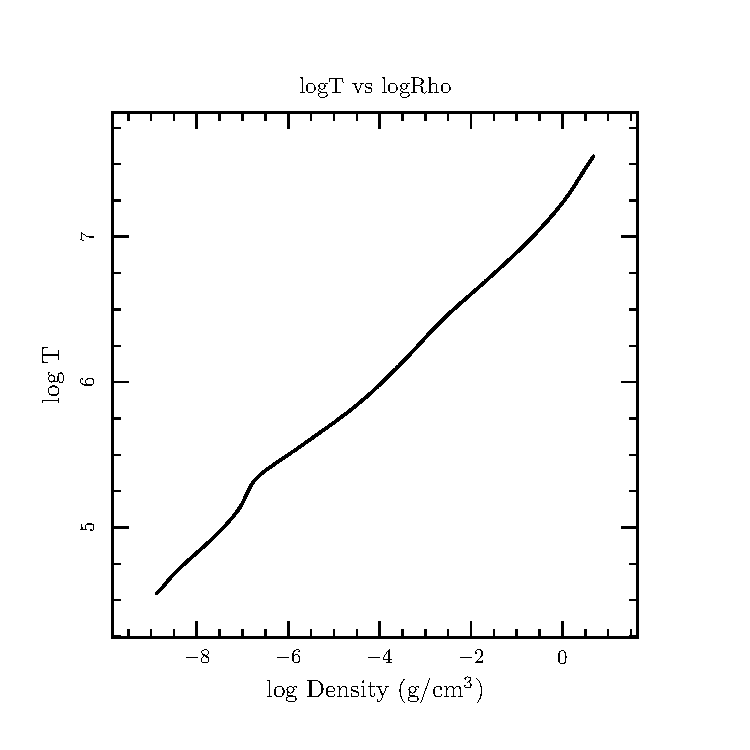
\includegraphics[width = 3.8in]{/Users/jaredbrooks/create_zams/plots_out/Log_T_vs_logRho.pdf}
	    \caption{}
	    \label{fig:1}
          \end{minipage}
          \hspace{0cm}
          \begin{minipage}[b]{0.5\linewidth}
            \centering
            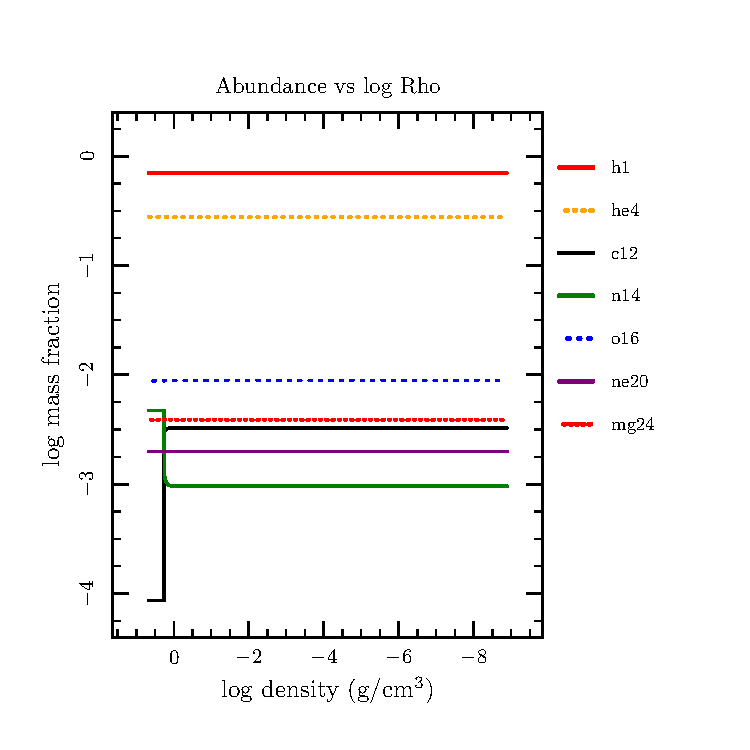
\includegraphics[width = 3.8in]{/Users/jaredbrooks/create_zams/plots_out/Abundance_vs_logRho.pdf}
            \caption{}
            \label{fig:2}
          \end{minipage}
	\end{figure}



\end{document}
